\section{Constrained Readout-Side Edit Test}
\label{app:lexical-control-stress-test}

This appendix reports a constrained readout-edit test for readout SAE decoder
directions, asking whether directions associated with a fixed
profanity-related candidate lexicon can move specified logit differences when edited at the
readout, and how that effect behaves under held-out terms, dose sweeps,
comparison rows, and off-target probes.

\begin{table*}[!tbp]
\caption{\textbf{Readout SAE decoder-direction edit summary.}
The constrained readout-side edit supports a readout-level intervention result: editing
SAE decoder directions selected from discovery tokens can move constrained lexical logit
differences. The table records the evidence used to pair intended margin shifts
with off-target lexical probes.}
\label{tab:lexical-control-stress-test}
\centering
\footnotesize
\setlength{\tabcolsep}{4pt}
\renewcommand{\arraystretch}{1.08}
\begin{tabularx}{\textwidth}{@{}p{0.18\textwidth}Y Y@{}}
\toprule
Measurement & What it measures & Setting \\
\midrule
Lexical specificity &
Degree to which the selected features and token summaries are associated with
the profanity-related lexical family instead of generic high-scoring rows. &
Supports feature selection for this edit test; feature ids remain the
stable objects and labels serve as token summary aids. \\
\addlinespace
Score-level intervention effect &
Whether editing along the selected SAE decoder directions changes the
specified profanity-vs-reference logit differences in the intended direction. &
Identifies a score-level effect at the edited readout; circuit tracing
\citep{ameisen2025circuittracing} can localize upstream sources. \\
\addlinespace
Held-out templates &
Whether the same intervention transfers to held-out lexical prompts and prompt
templates after feature selection. &
Measures held-out template transfer after feature selection. \\
\addlinespace
Dose response &
Whether larger intervention strengths produce ordered margin shifts before
quality or off-target behavior dominates. &
Measures dose ordering and separates threshold artifacts from graded response. \\
\addlinespace
Cross-model replication &
Whether the same intervention pattern appears in more than one
evaluated model. &
Replication is evidence for a recurring readout-level pattern, while each model
is reported alongside its own readout fidelity metrics. \\
\addlinespace
Off-target lexical probes &
Whether the intervention leaves unrelated lexical contrasts and neutral
prompts stable. &
These probes measure obvious off-target regressions alongside the intended
margin movement. \\
\addlinespace
Open-generation probes &
How the readout-level edit propagates when the model is allowed to generate
freely. &
Complements the candidate-constrained lexical-score measurements. \\
\bottomrule
\end{tabularx}
\end{table*}

\paragraph{Setup.}
The primary run uses Qwen3.5-2B with the 32$\times$, $k=256$ readout SAE
reported in Appendix~\ref{app:readout-factorizer-sweeps}. The evaluation vocabulary
contains 22 non-hateful profanity terms and 20 affect/control terms; all
single-token claims are filtered through the model tokenizer. Features are
selected from five discovery terms, \{\texttt{fuck}, \texttt{shit},
\texttt{hell}, \texttt{sucks}, \texttt{bastard}\}, and then evaluated on held-out
terms \{\texttt{fucking}, \texttt{fucked}, \texttt{bullshit}, \texttt{shitty},
\texttt{damned}, \texttt{asshole}, \texttt{bitch}, \texttt{crap},
\texttt{piss}, \texttt{pissed}\}. The intervention is a one-step logit edit:
for selected decoder directions \(d_f\), we add
\(v\WU^\top\) to the logits with
\(v=-\alpha\sum_{f\in F} d_f/\|d_f\|_2\). With this sign convention, positive
\(\alpha\) suppresses the selected profanity-associated directions. The reported
intervention scale is \(\alpha=16\). The primary candidate-constrained grid has
16 prompts, 9 profane-to-reference candidate pairs, 10 intervention scales, and 5 methods
(none, readout SAE direction edit, discovery token bias, oracle token bias, and
norm-matched random feature edit), giving 7200 evaluated rows.

\paragraph{Feature specificity.}
The selected directions are lexically specific: in the Qwen3.5-2B run, 12 of
the top 13 profanity-associated SAE features have
specificity \(1.0\) against the 20 control terms, and the remaining feature has
specificity \(0.988\). The token summaries partition recognizable lexical
families, including f-word, sh-word, hell/damn, and insult-related directions.
Feature ids remain the stable objects of analysis; token summary labels provide
the row-level description used for this edit test.

\begin{table*}[!tbp]
\caption{\textbf{Primary Qwen3.5-2B readout-edit comparison.}
All methods use intervention scale 16. Discovery token bias penalizes only the
five discovery token ids; oracle token bias penalizes the full evaluation lexicon.
Random features are norm-matched to the selected readout SAE direction edit.
\(\Delta p_{\mathrm{bad}}\) is reported as a positive reduction in probability
assigned to the profane-token side.}
\label{tab:lexical-control-primary-methods}
\centering
\scriptsize
\setlength{\tabcolsep}{4pt}
\renewcommand{\arraystretch}{1.08}
\begin{tabularx}{0.96\textwidth}{@{}lrrrrY@{}}
\toprule
Method & \makecell{Discovery\\flip} & \makecell{Held-out\\flip} &
\makecell{Held-out\\\(\Delta p_{\mathrm{bad}}\)} &
\makecell{Median\\KL} & Interpretation \\
\midrule
Readout SAE directions (10) & $0.450$ & $0.359$ & $0.398$ & $0.679$ &
Transfers from discovery terms to held-out variants. \\
\addlinespace
Discovery token bias & $0.450$ & $0.000$ & $0.000$ & $0.001$ &
Token-id edit restricted to discovery terms; held-out ids receive no direct bias. \\
\addlinespace
Oracle token bias & $0.450$ & $0.359$ & $0.404$ & $0.004$ &
Upper-bound token edit with full lexicon knowledge. \\
\addlinespace
Random features & $0.013$ & $0.156$ & $0.078$ & $1.363$ &
Norm-matched control with a different effect/cost profile. \\
\addlinespace
No intervention & $0.000$ & $0.000$ & $0.000$ & $0.000$ &
Reference condition. \\
\bottomrule
\end{tabularx}
\end{table*}

Table~\ref{tab:lexical-control-primary-methods} reports the key intervention
comparison: the readout SAE direction edit matches the oracle token bias held-out flip rate
while using only directions selected from discovery tokens, whereas the equally
informed discovery token bias has zero held-out effect. The match is exact
because scale 16 saturates the evaluation. A candidate can flip only when
the unedited model prefers the profane side, which holds for 23 of the 64
held-out and 36 of the 80 discovery candidates; at scale 16 the SAE
direction edit and the oracle flip exactly the same 23 held-out
candidates, so both rates equal the ceiling
\(23/64=0.359\) (cluster-bootstrap 95\% CI \(0.250\)--\(0.469\) for both
methods). The methods separate below saturation: at scale 4 the oracle
flips 20 of the 23 against the SAE edit's 11 (intersection 10), and the
oracle saturates by scale 6 while the SAE edit reaches the ceiling
at scale 12. KL summaries cluster at the prompt level, since
the 16 prompts are shared across both splits. The KL column records
the distributional cost of each edit. Across the intervention-scale sweep, the
discovery flip rate under the
readout SAE direction edit increases monotonically from \(0.038\) to
\(0.450\), and the held-out flip rate tracks it within about \(0.04\)
across the mid-range scales (6 to 10), widening to roughly \(0.07\) at
scale 4 and \(0.09\) at the headline scale 16.
The result establishes a constrained logit-difference intervention pattern;
open-generation behavior remains a separate evaluation layer beyond candidate
scoring.

\begin{table*}[!tbp]
\caption{\textbf{Cross-model readout SAE direction edit measurements.}
All rows use ten readout SAE decoder directions selected from discovery tokens at
intervention scale 16. Discovery directions are selected from five profanity tokens; held-out terms are
withheld from both the feature selector and the discovery-only token bias
baseline. The Ministral tokenizer leaves the held-out split below the
single-token threshold, so that row reports the discovery-side comparison.}
\label{tab:lexical-control-cross-model-results}
\centering
\scriptsize
\setlength{\tabcolsep}{3pt}
\renewcommand{\arraystretch}{1.08}
\begin{tabularx}{\textwidth}{@{}p{0.18\textwidth}p{0.19\textwidth}rrrrY@{}}
\toprule
Model & SAE used & \makecell{Feature\\discovery flip} &
\makecell{Feature\\held-out flip} & \makecell{Discovery-token\\bias held-out} &
\makecell{Off-target top1\\regression} & Setting \\
\midrule
Qwen3.5-2B &
32$\times$, $k=256$ &
$0.450$ & $0.359$ & $0.000$ & $0.444$ &
Primary readout-edit run. \\
\addlinespace
\shortstack[l]{R1-Distill\\Qwen-7B} &
32$\times$, $k=256$ &
$0.388$ & $0.469$ & $0.000$ & $0.222$ &
Same tokenizer family; reasoning-distilled checkpoint. \\
\addlinespace
\shortstack[l]{Ministral\\3-8B-Base} &
16$\times$, $k=128$ &
$0.562$ & -- & -- & $0.278$ &
Tokenizer-filtered held-out split; evaluated with an earlier strict SAE
checkpoint and reported as a discovery-side comparison. \\
\bottomrule
\end{tabularx}
\end{table*}

Table~\ref{tab:lexical-control-cross-model-results} records the quantitative
readout-edit outcome. The Qwen3.5-2B and R1-Distill-Qwen-7B rows show the
intended transfer pattern: the readout SAE direction edit transfers to held-out
lexical variants, while the discovery-only token bias baseline has zero
held-out effect because those token ids were not in its bias set. The Ministral
row provides a discovery-side cross-family comparison because its tokenizer leaves
too few held-out single-token terms for the held-out split.

The takeaway is positive: SAE decoder directions move constrained
lexical logit differences when edited at the readout; the intended
scores move under intervention, held-out templates and scale-sweep measurements
provide supporting evidence, and the two Qwen-family rows show the same
held-out lexical transfer pattern. The Ministral row is a discovery-side
cross-family comparison because too few held-out terms pass the tokenizer filter.
Off-target lexical probes map regressions beyond the intended candidate
scores: the Qwen3.5-2B off-target top-1 regression of \(0.444\)
(\Cref{tab:lexical-control-cross-model-results}) is the candidate-scoring
counterpart of the median-KL distributional cost, and marks the edit as
constrained in construction rather than in downstream effect.

\subsection{Matched-KL Frontier and Cross-Model Outcome}
\label{app:lexical-matched-kl}

The comparison above matches intervention scale; a stricter comparison
matches distributional cost. The upgraded protocol enlarges the held-out
lexicon from 64 to 240 candidates (12 held-out pairs \(\times\) 20
prompts), extends scales to 64 so that baseline frontiers reach SRP's KL
range, and adds three label-free control directions: the mean row of the
five discovery tokens, PCA rank-1, and PCA rank-4 (the full rank of the
discovery rows, hence capacity-fair); the oracle, discovery-bias, and
random brackets are retained. The frontier plots held-out suppression
(\(\Delta p_{\mathrm{bad}}\) primary, flip rate secondary) against
median next-token KL, and paired cluster bootstraps (same candidates
across methods; clustered conservatively by the 12 held-out terms and,
separately, by the 20 prompts; 10{,}000 resamples) test differences at
matched KL.

\begin{figure*}[!tbp]
    \centering
    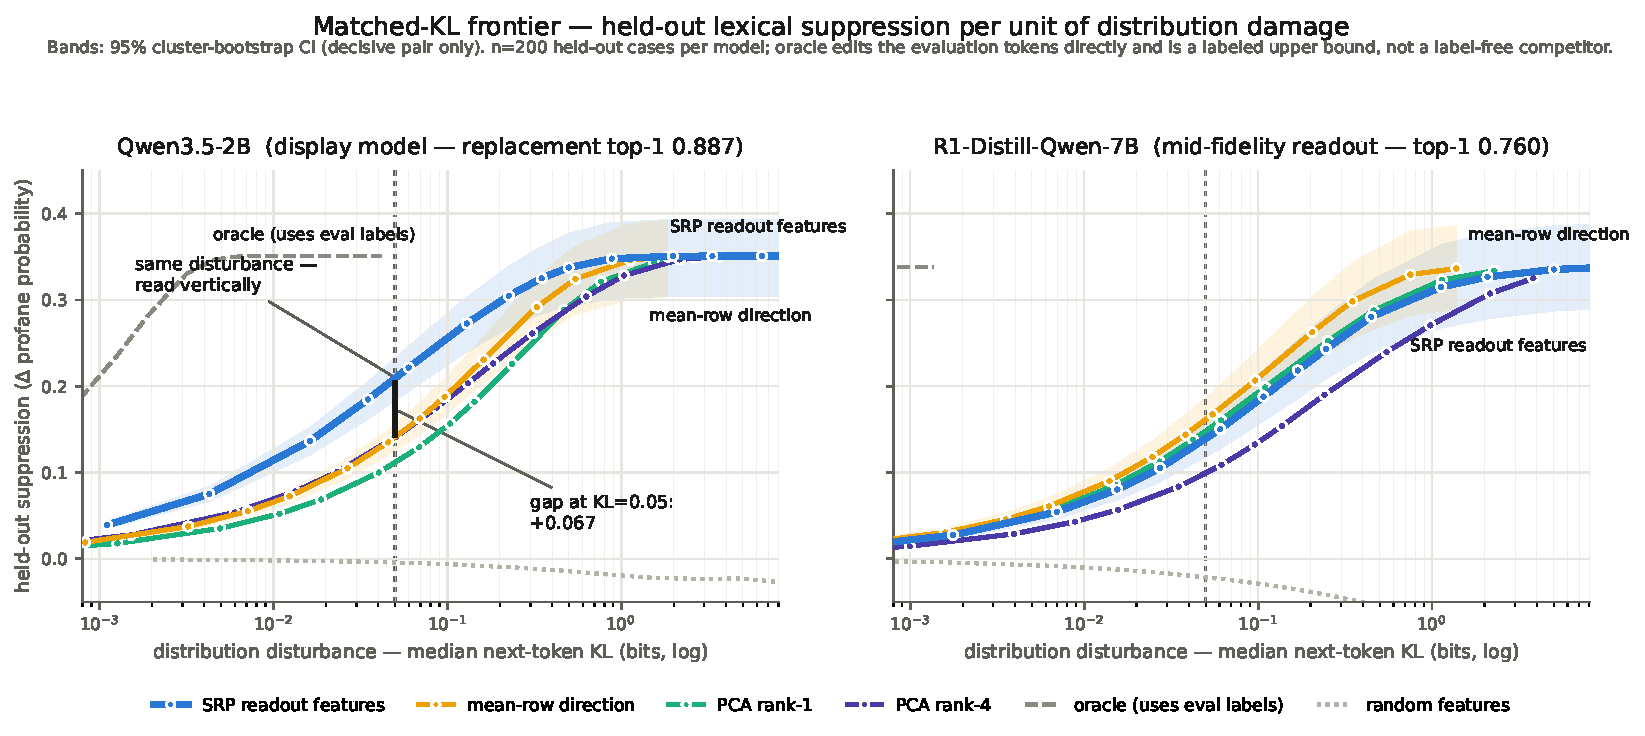
\includegraphics[width=0.86\textwidth]{figures/rebuttal/matched_kl_frontier_two_panel.pdf}
    \caption{\textbf{Held-out suppression versus distributional cost at
    matched KL (Qwen3.5-2B).} Held-out
    \(\Delta p_{\mathrm{bad}}\) (left) and flip rate (right) against
    median next-token KL for the SRP direction edit, mean-row, PCA
    rank-1/rank-4, and the oracle and random brackets. SRP dominates
    every label-free baseline at every matched KL on this model and
    reaches the oracle ceiling at scale 12; trivial directions reach it
    only at 1.3--5\(\times\) the KL.}
    \label{fig:lexical-matched-kl-frontier}
\end{figure*}

On the display model the outcome is decisive: SRP beats every label-free
baseline at every matched KL, with all 12 paired comparisons significant
(term-clustered CIs exclude zero). Against the strongest baseline, the
mean-row direction, the paired \(\Delta p_{\mathrm{bad}}\) advantage is
\(+0.032\) [\(+0.014\), \(+0.054\)] at KL 0.02, \(+0.087\)
[\(+0.065\), \(+0.115\)] at 0.05, \(+0.085\) [\(+0.062\), \(+0.109\)]
at 0.10, and \(+0.074\) [\(+0.048\), \(+0.103\)] at 0.20; against PCA
rank-4 the advantages span \(+0.036\) to \(+0.097\), all significant.

The advantage is model-specific, and we print the losses. At matched KL,
Qwen3.5-0.8B loses to the mean-row direction (\(\Delta\) \(-0.030\) to
\(-0.094\), significant) and Qwen3.5-9B loses more clearly (\(-0.086\)
to \(-0.135\), significant); R1-Distill-Qwen-7B is mixed (loses to
mean-row at two of four matched-KL points, beats PCA rank-4); Ministral
is excluded because the Tekken tokenizer leaves too few single-token
terms for feature discovery (the dictionary itself is validated in
Appendix~\ref{app:causal-validation}), and R1-Distill-Llama-8B is
excluded with one tokenizable pair and no held-out terms. Two candidate
explanations for the losses were tested and rejected: replacement
fidelity (the 9B readout is high-fidelity and still loses) and
dictionary width (a registered prediction that the narrower 0.8B
dictionary should win; it lost). The supported claim is therefore
scoped: on the display model, dictionary-direction edits beat trivial
category directions at matched distributional cost; the advantage is not
general across models, and mean-row is a strong label-free baseline.
